\documentclass[11pt]{article}

\usepackage[a4paper,margin=2.5cm,headheight=14pt]{geometry}
\usepackage[utf8]{inputenc}
\usepackage[T1]{fontenc}
\usepackage{fancyhdr}
\usepackage{graphicx}
\usepackage{xcolor}
\usepackage{listings}
\usepackage{hyperref}
\usepackage{enumitem}
\usepackage{amsmath}

\hypersetup{
    colorlinks=true,
    linkcolor=black,
    urlcolor=black,
    citecolor=black,
    pdftitle={Microcontrollers Project: Simon Says},
    pdfauthor={Jaime Esparragoso Vides}
}

\pagestyle{fancy}
\fancyhf{}
\renewcommand{\headrulewidth}{0.4pt}
\fancyhead[L]{Microcontrollers}
\fancyhead[R]{Simon Says Project}
\fancyfoot[C]{\thepage}

% ---- Code listing style (mimics the original document's look) ----
\definecolor{codebg}{HTML}{EDEDE3}
\definecolor{codegreen}{HTML}{2E7D32}
\definecolor{codeblue}{HTML}{1A56C4}
\definecolor{codepurple}{HTML}{8E24AA}
\definecolor{codegray}{HTML}{808080}

\lstdefinelanguage{CMSP}{
  language=C,
  morekeywords={interrupt,volatile,pragma,vector,uint16_t,uint32_t,int8_t,typedef}
}

\lstset{
  language=CMSP,
  backgroundcolor=\color{codebg},
  basicstyle=\ttfamily\footnotesize,
  keywordstyle=\color{codeblue}\bfseries,
  commentstyle=\color{codegreen},
  stringstyle=\color{codepurple},
  numberstyle=\tiny\color{codegray},
  numbers=left,
  numbersep=8pt,
  frame=single,
  rulecolor=\color{black!30},
  breaklines=true,
  breakatwhitespace=false,
  tabsize=2,
  showstringspaces=false,
  captionpos=b,
  columns=flexible,
  keepspaces=true
}

\title{\textbf{Microcontrollers Project:\\ Simon Says Game}}
\author{}
\date{}

\begin{document}

% ---------------- TITLE PAGE ----------------
\begin{titlepage}
\centering
\vspace*{1.5cm}
{\Huge \textbf{Microcontrollers Project:}\par}
\vspace{0.3cm}
{\Huge \textbf{Simon Says Game}\par}

\vspace{1.2cm}
{\large \textit{Bachelor's Degree in Electronic, Robotics and Mechatronics Engineering}\par}

\vspace{1.5cm}
{\large Author: Jaime Esparragoso Vides\par}

\vspace{0.8cm}
{\large Date: January 30, 2026\par}

\vspace{2cm}
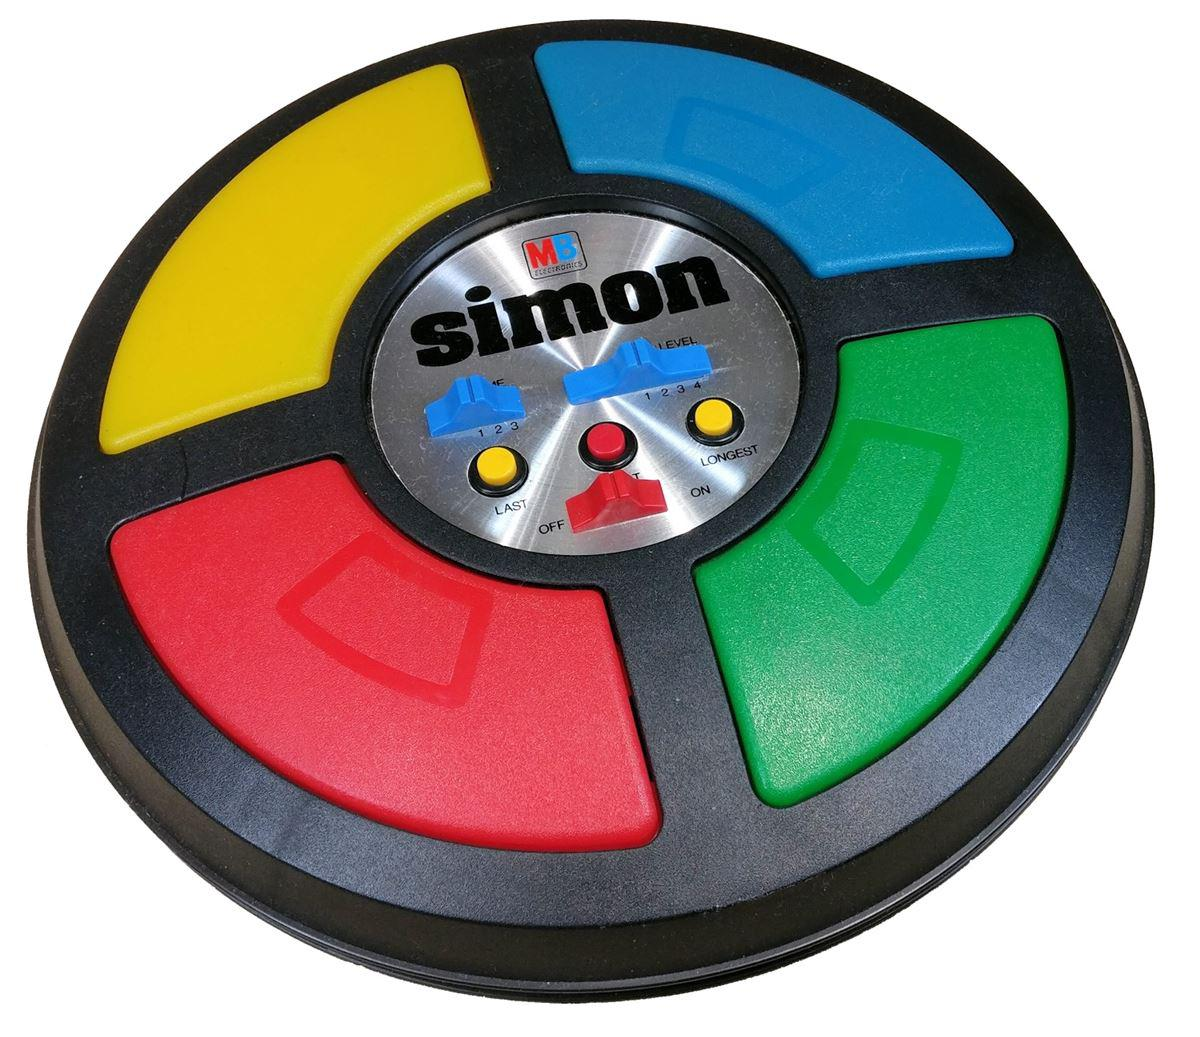
\includegraphics[width=0.5\textwidth]{img-000.jpg}

\vfill
{\large Universidad de Sevilla\par}
\vspace{1cm}
\end{titlepage}

% ---------------- TABLE OF CONTENTS ----------------
\tableofcontents
\newpage

% ==========================================================
\section{Introduction}

This report summarizes the development of our project for the course: we implement the classic ``Simon Says'' game using the MSP430 microcontroller and the BoosterPack MkII. The idea is to meet all the points proposed in the assignment, as specified in the example PDF.

% ==========================================================
\section{Hardware and Peripheral Configuration}

For this project we used libraries for the display, so that we could show whatever we wanted on the LCD screen. The rest of the functionality we implemented ourselves in the code:

\begin{itemize}
    \item \textbf{Joystick (ADC10):} We needed to continuously read the stick's position. We configured the ADC to read channels A0 and A3. The trickiest part here was calibrating the values: the joystick needs tolerance margins so the game doesn't detect phantom movements.

    \item \textbf{Timers:} We used two:
    \begin{itemize}
        \item \textit{Timer0:} Our main clock. It gives us an interrupt every 25 ms. This lets us time the rounds without using \texttt{delay()}, which is key because it means the microcontroller keeps detecting button presses while it ``waits''.
        \item \textit{Timer1:} Dedicated exclusively to audio. We use it in compare mode to output a PWM signal to the buzzer. By changing this timer's frequency on the fly we get the different musical notes.
    \end{itemize}

    \item \textbf{Interrupts:} For buttons S1, S2, and the joystick button, we use interrupts, which drive the behavior carried out by these inputs.

    \item \textbf{LCD Screen:} We use SPI communication, all handled inside the library. It is the most resource-intensive part, so we had to optimize the drawing code so it wouldn't slow down the game logic.
\end{itemize}

% ==========================================================
\section{Code Structure}

The structure we followed for our code is as follows:

\subsection{The Main Loop}

The core of the program (\texttt{main}) consists of an infinite loop (\texttt{while(1)}) that puts the microcontroller into low-power mode (\texttt{LPM0}) on every iteration. The system only ``wakes up'' through interrupts. The most important interrupt is \textbf{Timer0}'s, configured to fire every 25 milliseconds. This interrupt raises a global flag called \texttt{tick}.

\begin{itemize}
    \item If \texttt{tick == 0}: The processor sleeps, saving power.
    \item If \texttt{tick == 1}: The main loop runs one cycle of game logic, updates counters, and goes back to sleep.
\end{itemize}

\subsection{State Machine (FSM)}

To manage the game logic, we implemented a State Machine controlled by the \texttt{estado} variable. The defined states (\texttt{estados\_t}) are:

\begin{enumerate}
    \item \textbf{BIENVENIDA:} Initial idle state. Waits for the player to press ``Start''. Plays a looping melody and checks whether ``Symbol Mode'' is activated.
    \item \textbf{MENSAJE\_RONDA:} Transition state that clears the screen and announces the current round number to the player.
    \item \textbf{MAQUINA:} The system steps through the \texttt{secuencia} array and lights up the corresponding colors/symbols.
    \item \textbf{TURNO\_JUGADOR:} The system waits for input from the ADC (joystick). It compares the user's input against the stored sequence. If there is an error or the time runs out (\textit{timeout}), we move to \texttt{FIN}. If the sequence is completed, we move to \texttt{VICTORIA}.
    \item \textbf{VICTORIA:} We show an animation and success music after clearing a round.
    \item \textbf{VICTORIA\_FINAL:} State reached after clearing all 32 rounds. Shows a star animation and increases the difficulty.
    \item \textbf{FIN:} ``Game Over'' screen; shows the final score and allows restarting.
\end{enumerate}

% ==========================================================
\section{Detailed Description of Functions and Constants}

A brief expansion on some of the constants and functions declared:

\subsection{Definitions and Constants (\texttt{\#define})}

Macros were mainly used for two purposes: music and graphics.

\begin{itemize}
    \item \textbf{Musical Notes:} We defined the note frequencies (e.g. \texttt{\#define DO 262}, \texttt{\#define LA 440}). This makes writing melodies in the code much simpler and more intuitive.
    \item \textbf{Hexadecimal Colors:} The graphics library uses 32-bit values. We defined constants such as \texttt{GRAPHICS\_COLOR\_BRIGHT\_GREEN} so we could create our own custom colors.
    \item \textbf{Animation Parameters:} Constants such as \texttt{N\_VICTF} or \texttt{N\_ESTRELLAS} control the length of the melodies and the number of little stars on screen.
\end{itemize}

\subsection{Critical Global Variables}

Because Interrupt Service Routines (ISRs) cannot return values, we use \texttt{volatile} global variables for communication between the interrupts and the main loop:

\begin{itemize}
    \item \texttt{volatile unsigned char tick}: This variable is the system's main clock.
    \item \texttt{volatile unsigned char start}: Indicates whether the joystick button has been pressed.
    \item \texttt{lfsr}: 16-bit shift register for the pseudorandom number generator.
\end{itemize}

\subsection{Initial Functions}

These functions isolate the game logic from the MSP430-specific registers, making the code more portable and readable.

\begin{description}
    \item[\texttt{Set\_Clk(char VEL)}] Configures the timer to run at 1, 8, or 16 MHz. For this game, we set it to 16 MHz.
    \item[\texttt{inicia\_ADC(char canales)} and \texttt{lee\_ch(char canal)}] Configure the ADC and read its value.
    \item[\texttt{init\_buzzer()}, \texttt{suena\_hz()} and \texttt{apaga\_sonido()}] Control Timer1.
    \begin{itemize}
        \item \texttt{suena\_hz} calculates the value of the \texttt{TA1CCR0} register based on the desired frequency, to generate a square-wave (50\% PWM) signal.
        \item \texttt{apaga\_sonido} stops the timer to silence the system.
    \end{itemize}
\end{description}

\subsection{Logic and Algorithm Functions}

\begin{description}
    \item[\texttt{lfsr\_siguiente()} and \texttt{aleatorio\_1\_4()}] Implement the pseudorandom number generator (Requirement 2.3). We use an LFSR (Linear Feedback Shift Register) algorithm that generates a random sequence to play with.
    \item[\texttt{dibuja\_estrella()}] A graphics helper function that draws shapes at random (x,y) coordinates for the final-victory animation.
\end{description}

% ==========================================================
\section{Requirements Implementation}

Below, we detail how we translated each point of the assignment into our C code:

\subsection{General Features and Accessibility (Items 1.x)}

\begin{itemize}
    \item \textbf{Colors and Sounds (1.1):} We defined the frequencies (\texttt{\#define DO 262}, etc.) and the colors in arrays (\texttt{color\_alto[]} and \texttt{color\_bajo[]}). This lets us work with them easily.

    \item \textbf{Colorblind Mode (1.2):} In the start routine, we also check whether the player is holding the joystick to the left (\texttt{ejex < 100}). If so, we set a flag \texttt{modo\_simbolos = 1}. From that point on, all drawing logic splits into two paths: it either draws colors, or it draws the characters \#, @, \$ and \% on a black background.

    \item \textbf{Timing (1.3):} The game's timings are not fixed, but variable. We compute \texttt{T} and \texttt{T4} based on a \texttt{tiempo\_base} variable (1000 ms at the start). The state machine uses counters (\texttt{tms}) that increment on every timer tick.

    \item \textbf{Visual Feedback (1.4):} To simulate ``lighting up'', we redraw the same rectangle but change the color from \texttt{color\_bajo} to \texttt{color\_alto}.
\end{itemize}

\subsection{Random Generation (Items 2.x)}

\begin{itemize}
    \item \textbf{Random Sequence (2.3):} To comply with the restriction, we do not use \texttt{stdlib.h} for randomness. We use a 16-bit LFSR (Linear Feedback Shift Register) in the \texttt{lfsr\_siguiente()} function. Through XOR operations and bit shifts, we obtain a pseudorandom sequence.

    \item \textbf{Human Seed (2.2):} To make every playthrough unique, the initial seed (\texttt{lfsr}) is loaded with the value of \texttt{contador\_ticks} when the player presses the Start button.

    \item \textbf{Cumulative Sequence (2.5):} We use a single \texttt{secuencia[32]} array. In round 1, the machine reads up to index 0; in round 2, up to index 1, and so on. We do not generate a new sequence every round; instead we reuse the initial sequence of 32 terms.
\end{itemize}

\subsection{Interface and Game Flow (Items 3, 4 and 5)}

\begin{itemize}
    \item \textbf{Game States:} We split the flow into clear states:
    \begin{itemize}
        \item \texttt{BIENVENIDA}: The opening melody plays and it waits for the button.
        \item \texttt{MENSAJE\_RONDA}: Shows the current round number.
        \item \texttt{MAQUINA}: Plays back the sequence using the \texttt{secuencia} array and the timer.
        \item \texttt{TURNO\_JUGADOR}: Reads the joystick. If the player takes longer than \texttt{2*T} (controlled by \texttt{tms >= T2}), it jumps to \texttt{FIN}.
    \end{itemize}

    \item \textbf{Score (5.7):} We compute the score step by step. Every correct answer increments the \texttt{puntuacion} variable. This means that if you fail partway through a round, you still keep the points for the steps you got right.

    \item \textbf{Hard Mode (5.5):} If the player clears all 32 rounds, the game enters \texttt{VICTORIA\_FINAL}. If Start is pressed again, we restart the game by setting \texttt{modo\_rapido = 1}, which halves the base time, making the game twice as fast.
\end{itemize}

\subsection{High Scores and Improvements}

We were not able to make progress on this part due to the board's limited resources, since at a certain point it started throwing errors and displaying random colors (video attached). We do have the code for how we implemented the high-score screen to save them, even though it ended up being on an external one.

% ==========================================================
\section{Source Code}

Below is the complete code implemented for the project:

\lstinputlisting[caption={Complete code for the Simon Says game (main.c)}]{main.c}

\end{document}
